\section{Introduction}

ELCC enables statistical analyses to be performed across an unprecedented variety of emergent language corpora with ease.
Nevertheless, the fact that corpora of ELCC only contain utterances with no accompanying context severely limits the range of analyses that can performed in the grand scheme of emergent communication research.
The surrounding context of the utterance is necessary for investigating the semantics of utterances which in turn are necessary for understanding the syntax, pragmatics, and broader social context of the utterance---all major areas of interest for emergent communication research.
Thus, we propose ELCC Plus which expands upon ELCC primarily by adding context to each utterance in the corpora, capturing information such as the
  state of the world,
  identity of the speaker,
  the speaker's observation,
  the previous and following timesteps,
  and the progress in the overall optimization process.
Providing this additional context in an easily-accessible format based on ELCC will enable a wide range of analyses from the emergent communication literature to be performed directly on the static data without needing to spin up an emergent communication system directly.


\paragraph{Related work}
The most closely related work comes from the standardized reinforcement learning toolkits PettingZoo \citep{terry2021pettingzoo} and Minari \citep{minari}.
  \unskip\footnote{Both of these are projects of the Farama Foundation which also maintains Gymnasium, the somewhat official continuation of OpenAI Gym.}
\citet{terry2021pettingzoo} introduce the Agent--Environment Cycle (AEC) formalism to describe an API for multiagent reinforcement learning environments with a significant amount of generality.
AEC, and consequently the API of PettingZoo, should, in theory, be able to express emergent communication environments.
Leveraging this formalism and API would improve interoperability with existing tools in the RL ecosystem, but it could also come at a cost of naturally expressing emergent communication environments.
Minari, on the other hand, is a toolkit for offline RL, including the serialization of trajectories (a.k.a., episodes, rollouts) into static datasets.
Minari currently does not have any support for PettingZoo/AEC or any other multi-agent environments.
Nevertheless, its serialization techniques will be relevant even if the codebase is not used directly.



\section{Format}

When designing the format for the rich corpora, there are two primary goals in representing the episodes in the emergent communication systems.
The first goal is to completely and accurately represent what happens in the episode.
The second is to do so in a consistent format with consistent interpretations of the elements of the format.
Due to the diverse ways in which ECSs can vary, this is a difficult, if not impossible, goals to achieve with a simple, static serialization.
Completely representing each ECSs would result in largely inconsistent formatting while adhering to stricter formatting would result in a lossy storage of the ECS episodes.

Thus, we propose a two-part format for representing the corpora of ELCC Plus.
The first part is a serialization of the episodes/trajectories unique to each ECS, while the second part is a collection of (Python) functions which provide a consistent interface to various parts of the corpus.
In particular, the serialization will capture as much information as possible about each episode, adhering to conventions (e.g., utterances are always referred to as ``utterance'', not ``message'' while not being limited to a particular format (e.g., each timestep could have one, zero, or many utterances).
While the serializations will be as consistent as possible, the level of variation required to accurately represent an ECS episode will require programmatic adapters to provide a consistent interface for the elements the ECSs do have in common.
This approach yields the best of both worlds:
  the ECS-specific serialization format allows as much information to be represented as possible in a way that corresponds well to the environment while the adapter-based interface allows for easy extraction of relevant data across the variety of corpora.
Furthermore, this format is extensible since new adapters can be written to extend the interface without needing to rerun the underlying ECS\@.


\subsection{Concrete Example}

\paragraph{Environments}

\begin{figure}
  \centering
  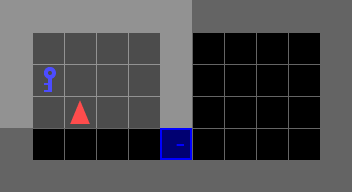
\includegraphics[height=1.5in]{chapters/elcc-plus/assets/babyai}
  \caption{A visualization of the Minigrid (f.k.a., BabyAI) navigation environment \protect\citep{chevalier2018babyai,MinigridMiniworld23}.}
  \unskip\label{fig:minigrid}
\end{figure}

In order to illustrate the format of the enriched collection, we will use two environments.
The first environment is the discrimination variant the signalling game where the observations are concatenations of one-hot vectors.
The second environment is a sender--receiver navigation based on Minigrid framework.
In this game, the receiver is an embodied agent in a grid world environment who must navigate to the goal based on messages from the sender who can observe the whole environment (illustrated in \Cref{fig:minigrid}).
Additionally, there is a one-to-many relationship between messages and actions the receiver takes, that is, the receiver may take multiple steps before the sender sends another message.


\paragraph{Serialization}
In \Cref{fig:serialization}, we present a simplified serialization of episodes in the signalling game and navigation environments.
For the signalling game, the serialization is relatively straightforward since every episode consists of a single timestep with the same components;
  there are observations and actions made by the sender and the receiver, a reward given by the environment, and other metadata like the step in the optimization process.
The navigation environment has more moving parts, and the serialization is, as a result, more complicated.
The observations themselves have more information and structure compared to the single vector in the signalling game.
More important to studying communication, though, is the fact that there are multiple time steps in the environment which themselves potentially contain utterances.

Even in this simple example, it is evident that coming up with a strict data format for serializing emergent communications systems would difficult and cumbersome.
The signalling game only consists trivially of one or two steps, and it is much more natural to represent as not having any steps at all.
Meanwhile the navigation environment requires being broken into a variable number of steps.
If we were to try to serialize a multi-agent navigation environment, we would no longer able to simply refer to the {\small\texttt{utterance}} or {\small\texttt{receiver\_action}} of each step and instead would have to generalize the representation to multiple utterances and actions per step.
This list of generalization can go on indefinitely, and so it is the best interest of the collection to keep this part of the representation flexible so as to not limit the future scope of the collection.


\begin{figure}
  \centering
  \begin{subfigure}[t]{0.4\linewidth}
    \centering
    \footnotesize
\begin{verbatim}




- optimization_step: 100
  reward: 1.0
  utterance: [3, 1, 4, 1]
  observation:
    sender: [1, 0, 1, 0]
    receiver:
      - [1, 0, 0, 1]
      - [1, 0, 1, 0]
      - [0, 1, 0, 1]
  correct_idx: 1
  receiver_action: 1

- optimization_step: 101
  reward: 0.0
  utterance: [1, 2, 3, 4]
  observation:
    sender: [1, 0, 0, 1]
    receiver: ...
  correct_idx: 1
  receiver_action: 0




\end{verbatim}
    \caption{Basic signalling game}
  \end{subfigure}
  \hfill
  \begin{subfigure}[t]{0.4\linewidth}
    \centering
    \footnotesize
\begin{verbatim}
- optimization_step: 100
  reward: 0.0
  steps:
    - map:
        walls: ...
        key: ...
        receiver: ...
        door: ...
        goal: ...
      utterance: [1, 1, 2, 2]
      receiver_action: move
      observation:
        sender: ...
        receiver: ...
      stop: false

    - map: ...
      utterance: null
      receiver_action: pick_up
      observation: ...
      stop: false

    - map: ...
      stop: true

- optimization_step: 101
  reward: 1.0
  steps: ...
\end{verbatim}
    \caption{Multi-step navigation game based on Minigrid environment}
  \end{subfigure}
  \caption{Example representations of two different emergent communication environments.  Format is based on YAML\@.}
  \unskip\label{fig:serialization}
\end{figure}


\paragraph{Interface}


\begin{figure}
  \centering
  \begin{subfigure}[t]{0.4\linewidth}
    \centering
    \footnotesize
\begin{verbatim}
def utterances(episodes):
  for ep in episodes:
    yield ep.utterance

def semantics_sender(episodes):
  for ep in episodes:
    yield ep.observation.sender

def semantics_receiver(episodes):
  for ep in episodes:
    idx = ep.receiver_action
    yield ep.observation.receiver[idx]
\end{verbatim}
    \caption{Signalling game}
  \end{subfigure}
  \hfill
  \begin{subfigure}[t]{0.55\linewidth}
    \centering
    \footnotesize
\begin{verbatim}
def utterances(episodes):
  for ep in episodes:
    for step in ep.steps:
      if step.utterance is not null:
        yield step.utterance

def semantics_sender(episodes):
  for ep in episodes:
    for step in ep.steps:
      if step.utterance is not null:
        yield ep.utterance, ep.observation.sender

def semantics_receiver(episodes):
  for ep in episodes:
    actions = []
    utterance = ep.steps[0].utterance
    for step in ep.steps:
      if step.utterance is not null or step.stop:
        yield utterance, actions
        actions = [step.receiver_action]
      else:
        actions.append(step.receiver_action)
\end{verbatim}
    \caption{Navigation game}
  \end{subfigure}
  \caption{Python pseudo-code for interfaces corresponding to the serializations in \Cref{fig:serialization}.}
  \unskip\label{fig:interface}
\end{figure}

The interface we will introduce for illustration purposes will consist of three elements which provide:
  (1) the utterances alone,
  (2) utterances with meaning the sender is trying to convey,
  and (3) utterances with the meaning as interpreted by the receiver.
While these elements are simple, the demonstrate nicely how the implementations adapt the variability in the serialization the uniformity required by the interface.
We give Python pseudo-code for the implementation of this interface in \Cref{fig:interface}.

The interface implementation for the signalling game is, again, relatively straightforward due to the simplicity of the environment and, in turn, serialization.
On the other hand, the implementations for the navigation environment have to account for more variability and nuance.
Firstly, the implementations for the utterances as well as utterances plus sender meaning requires that steps without utterances be filtered out.
More interestingly, the receiver-side semantics implementation requires aggregating the actions the receiver takes over multiple timesteps as the interpretation of the sender's utterance may entail taking a sequence of actions.

One could easily quibble here with the interpretation of ``meaning'' in the interface's implementations, but this illustrates an important benefit of the two-part representation proposed.
So long as the initial serialization format is expressive enough for a given emergent communication system, the more nuanced discussions (e.g., what constitutes a meaning in this environment?) can take place at the level of the interface's implementation (or initial definition).
Importantly, this does not require rerunning the emergent communication system and recollecting the data; rather, the implementation of the interface can be edited as necessary and be rerun over the serialization (which is comparatively cheap computationally to running a deep learning-based multi-agent simulation).


\subsection{Contents}
The contents of the enhanced corpora collection will largely overlap with ELCC, as the implementations for those emergent communication systems have already been verified as runnable.
The contents of this collection, though, will be extended, as necessary, to illustrate elements of the interface as well as to provide meaningful data for the experiments illustrating the utility of the proposed collection and its format.


\section{Experiments}

The experiments for this chapter will primarily demonstrate how it is possible to compute a wide range of metrics from the emergent communication literature based on the ELCC Plus.
These experiments will highlight that ELCC Plus enable performing a rich set of analyses over a variety of emergent languages based on static data.
This breaks the current paradigm of usually needing to run the emergent communication system itself in order to generate the required data for analyses involving the semantics of emergent communication.
The following metrics are proposed.
\begin{itemize}
  \item \emph{Topographical similarity}\quad
    quantifies compositionality by measuring correlation between pairwise distances in the message space and pairwise distances in the meaning space.
    Also known as \emph{toposim}.
    \citep{brighton2006UnderstandingLE,lazaridou2018emergencelinguisticcommunicationreferential}
  \item \emph{Instantaneous coordination}\quad
    measures the effect that one agent's actions have on another's actions in a multi-agent environment.
    It is quantified as the mutual information between the utterances of a first agent and the action of a second agent at the next timestep.
    \citep{jaques2019social}
  % \item \emph{Utility-informativeness-complexity}\quad
  %   is a trio of metrics derived from information bottleneck theory \cmt{check this} and information theory more generally.
  %   Each of these is defined in terms of entropy with
  %   \cmt{cite}
  \item \emph{Diachronic features}\quad
    refer to any metric that is tracked over the course of the optimization process.
    For example, the entropy of communication may start with a high entropy as it is mostly random but gradually decrease as the agents develop a communication protocol with a limited number of expressions.
  \item \emph{Ease-of-teaching}\quad
    measures how quickly and effectively an emergent language is acquired by new member in a dynamic population of agents.
    \citep{li2019ease}
\end{itemize}
